% !TEX TS-program = pdflatexmk
\documentclass[addpoints,10pt]{exam}

% Include custom style files
\usepackage{commands}
\usepackage{environments}

\usepackage{psfrag}
\usepackage[dvips]{epsfig}
\usepackage{epsfig}
\usepackage{color}
\usepackage{enumitem}
\usepackage{hyperref}
\usepackage{cleveref}
\usepackage[utf8]{inputenc}
\usepackage{mathtools}

\usepackage{algorithm,algorithmic}
\newcommand{\nb}[3]{{\colorbox{#2}{\bfseries\sffamily\scriptsize\textcolor{white}{#1}}}{\textcolor{#2}{\sf\small\textit{#3}}}}
\begin{document}
\thispagestyle{plain}

% parenthesis
\newcommand{\autopar}[1]{{\left(#1\right)}}
\newcommand{\automedpar}[1]{{\left[#1\right]}}
\newcommand{\autobigpar}[1]{{\left\{#1\right\}}}
\newcommand{\autoabs}[1]{{\left|#1\right|}}
\newcommand{\autonorm}[1]{{\left\|#1\right\|}}
\newcommand{\autoprod}[1]{{\left\langle#1\right\rangle}}

% comments

%%%%%%%%%%%%%%%%%%%%%%%%%%%%%%%%%%%%%%%%%%%%%%%%%%%%%%%%%%%%%%%%%%%%%%
\vspace*{-1.5cm}
{\noindent \rule{15.8cm}{.3mm} \\}
\begin{center} \bf
{\Large Foundations of Reinforcement Learning \medskip
\\
Assignment 2 \medskip}
\\ Issue date: November 09, 2021
\\ Due date: November 26, 2021
\\ 
\end{center}
\rule{15.8cm}{.3mm} \\[0cm]
\setlength{\parindent}{0pt}
%\pagenumbering{gobble}
\pagestyle{empty}
\global\hyphenpenalty=100000 
%%%%%%%%%%%%%%%%%%%%%%%%%%%%%%%%%%%%%%%%%%%%%%%%%%%%%%%%%%%%%%%%%%%%%%

\textbf{Coverage:} Value-based methods, policy gradient methods \medskip


\section*{Instructions}
\begin{itemize}
    \item \emph{Where to submit:} Please submit your solution as a PDF on Moodle. File name should follow the format \texttt{Assignment2-Lastname-Firstname.pdf}. 
    
    \item \emph{How to write solutions:} You should type your solution using LaTeX and following the template. Handwritten solutions will not be graded. Keep in mind the following premise: 
    \begin{itemize}
        \item[-] When writing in English, write short, simple sentences.
        \item[-] When writing a proof, write clear, precise statements. 
    \end{itemize}
    You can use previous points of the same problem without proving them. You can use results from the lectures if you reference them properly.
       
    \item \emph{Discussion:} You may discuss only at a high level with classmates. You should not dig around for homework solutions; if you do rely upon external resources, cite them, and write solutions in your own words. We ask you to please follow the ETH Disciplinary Code. 

    
    \item \emph{Grading:} Grading will be based on the completeness and correctness of your solution according to points assigned for each exercise. \texttt{Final grade = min(regular points + bonus points, 100)}.

    We reserve the right to deduct points on sloppy \LaTeX, minor errors in calculations, and unclear writing in general.
    
    \item \emph{Re-grading:} You may request for regrading within one week after the grade is released, with a written justification of why your solution deserves more points.

     
    \item \emph{Encountering problems?} 
    \begin{itemize}
        \item If you think some exercise is unclear or wrong use the Forum \textit{Assignments} in Moodle or reach out to the TA in charge of the exercise. 
        \item If you have trouble submitting your solution to Moodle within six hours before the deadline due to technical problems, you can send your PDF solution to our head TA. 
    \end{itemize}
\end{itemize}

%==========================================================================================================

\newpage
%==========================================================================================================

\section{Monte Carlo and TD Learning (20 Points)}

Consider a Markov Decision Process $\mathcal{M} = (\mathcal{S}, \mathcal{A},\mathcal{P}, r, \mu, \gamma)$ with deterministic dynamics, and a state space $\mathcal{S}=\{A, B, T\}$, where $T$ is a terminal state. As shown in the figure below, in state $A$ the agent can perform two actions: stay at $A$ (``stay") with reward $1$ or leave to $B$ (``switch") with reward $0$. In state $B$ there are two actions: go back to $A$ (``switch") with reward $1$ or leave for $T$ ("stay") with reward $2$ and the episode terminates. Let the discount factor be  $\gamma = 0.5$. 
  
\begin{center}
    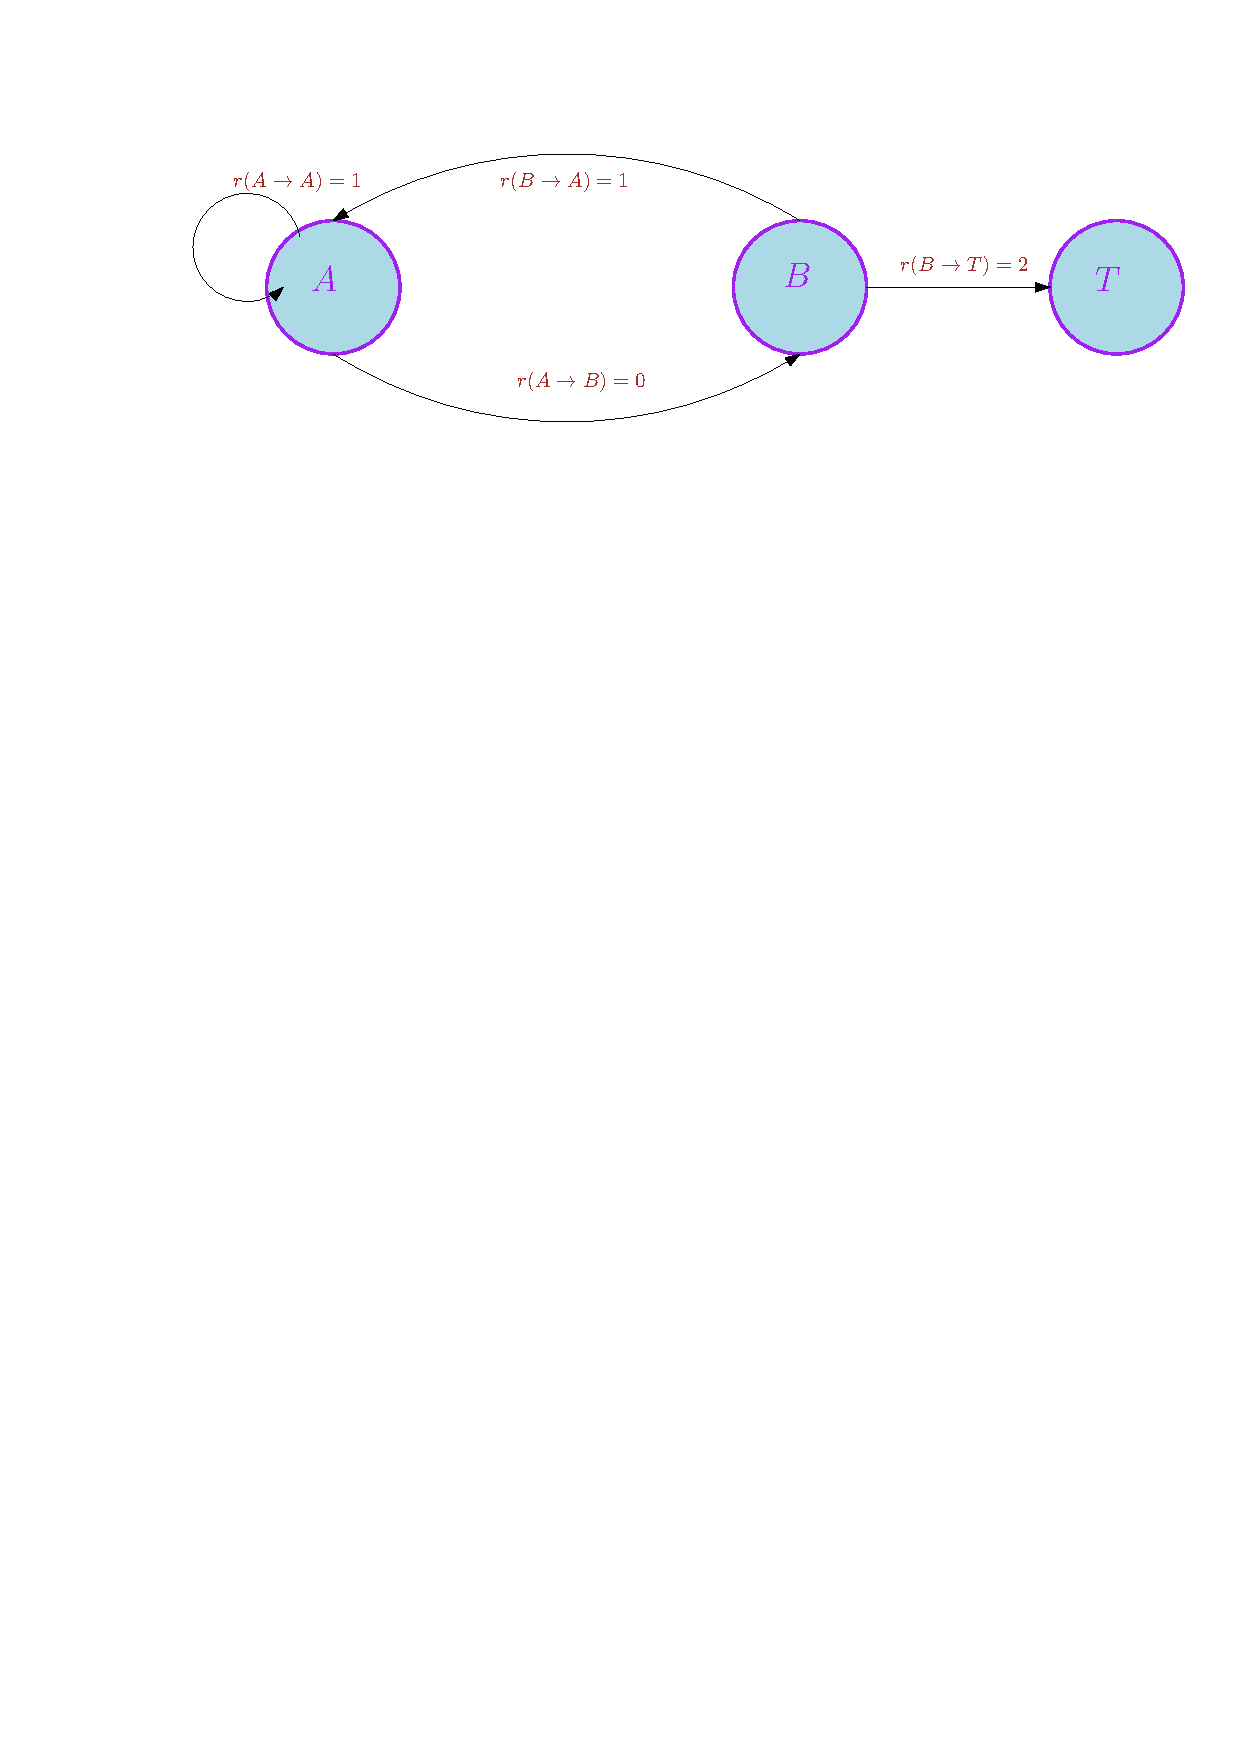
\includegraphics[width=0.6\linewidth]{figs/mdp_3state.pdf}
\end{center}
\vspace{8pt}


In other words, we have $\mathcal{S}=\{A,B,T\}$, $\mathcal{A}=\{\text{switch}, \text{stay}\}$,
$$
r(A,\text{switch})=0,\ \ r(A,\text{stay})=1,\ \ r(B,\text{switch})=1,\ \ r(B,\text{stay})=2,
$$
$$
P(B|A,\text{switch})=1,\ \ P(A|A,\text{stay})=1,\ \  P(A|B,\text{switch})=1,\ \ P(T|B,\text{stay})=1.
$$

\begin{questions}
    \question[10]  Consider the following three trajectories $[A, A, B, T]$, $[A, B, A, B, T]$ and $[A, B, T]$ sampled from an unknown policy $\pi$. Estimate $V^\pi(A)$ with first-visit MC (first-visit MC method  averages the returns following first visits to $s$) and every-visit MC (every-visit MC method averages the returns following all visits to $s$)\footnote{Refer to \cite[Section 5.1]{sutton2018reinforcement} for details.}.
    \question[10] Observe the trajectory: $[A, B, A, A, B, T]$. Compute the state(-action) value functions $V(s)$ (or $Q(s, a)$) after observing this trajectory and applying:
    \begin{itemize}
        \item TD(0);
        \item 2-step TD;
        \item SARSA;
        \item Q-learning.
    \end{itemize}
    The value function is initialized to $0$ in each state, and the learning rate is $\alpha = 0.1$. Compute it in an online-fashion, i.e. update the value every time you see a new state and reward, and show the detailed steps. 
\end{questions}



Contact: \texttt{junchi.yang@inf.ethz.ch}

\begin{Solution}
\begin{enumerate} [label=\alph*)]
        \item
        \textbf{First-visit MC}
        
        Episode $[A, A, B, T]$
        $$
        \begin{aligned}
        G_1 & = r(A,\text{stay}) + \gamma r(A,\text{switch}) + \gamma^2 r(B,\text{stay}) \\
        & = 1 + 0.5 \cdot 0 + 0.5^2 \cdot 2 \\
        & = 1.5
        \end{aligned}
        $$
        
        Episode $[A, B, A, B, T]$
        
        $$
        \begin{aligned}
        G_2 & = r(A,\text{switch}) + \gamma r(B,\text{switch}) + \gamma^2 r(A,\text{switch}) + \gamma^3 r(B,\text{stay}) \\
        & = 0 + 0.5 \cdot 1 + 0.5^2 \cdot 0 + 0.5^3 \cdot 2 \\
        & = 0.75
        \end{aligned}
        $$

        Episode $[A, B, T]$
        
        $$
        \begin{aligned}
        G_3 & = r(A,\text{switch}) + \gamma r(B,\text{stay}) \\
        & = 0 + 0.5 \cdot 2 \\
        & = 1
        \end{aligned}
        $$
        
        Thus
        $$
        V^\pi(A) = \dfrac{1}{3} (G_1 + G_2 + G_3) = \dfrac{13}{12}
        $$
        
        \vspace{1em}
        \textbf{Every-visit MC}
        
        Episode $[A, A, B, T]$
        $$
        \begin{aligned}
        G_{11} & = r(A,\text{stay}) + \gamma r(A,\text{switch}) + \gamma^2 r(B,\text{stay}) \\
        & = 1 + 0.5 \cdot 0 + 0.5^2 \cdot 2 \\
        & = 1.5 \\
        G_{12} & = r(A,\text{switch}) + \gamma r(B,\text{stay}) \\
        & = 0 + 0.5 \cdot 2 \\
        & = 1
        \end{aligned}
        $$
        
        Episode $[A, B, A, B, T]$
        
        $$
        \begin{aligned}
        G_{21} & = r(A,\text{switch}) + \gamma r(B,\text{switch}) + \gamma^2 r(A,\text{switch}) + \gamma^3 r(B,\text{stay}) \\
        & = 0 + 0.5 \cdot 1 + 0.5^2 \cdot 0 + 0.5^3 \cdot 2 \\
        & = 0.75 \\
        G_{22} & = r(A,\text{switch}) + \gamma r(B,\text{stay}) \\
        & = 0 + 0.5 \cdot 2 \\
        & = 1
        \end{aligned}
        $$

        Episode $[A, B, T]$
        
        $$
        \begin{aligned}
        G_{31} & = r(A,\text{switch}) + \gamma r(B,\text{stay}) \\
        & = 0 + 0.5 \cdot 2 \\
        & = 1
        \end{aligned}
        $$
        
        Thus
        $$
        V^\pi(A) = \dfrac{1}{5} (G_{11} + G_{12} + G_{21} + G_{22} + G_{31}) = \dfrac{21}{20}
        $$
        \vspace{1em}
        
        \item
        \textbf{TD(0)}
        $$
        V(A) \leftarrow 0, \quad V(B) \leftarrow 0
        $$
        
        [$t = 0: s_t = A, s_{t+1} = B$]
        $$
        V(A) \leftarrow V(A) + \alpha (r(A,\text{switch}) + \gamma V(B) - V(A)) = 0 + 0.1(0 + 0.5 \cdot 0 - 0) = 0
        $$
        [$t = 1: s_t = B, s_{t+1} = A$]
        $$
        V(B) \leftarrow V(B) + \alpha (r(B,\text{switch}) + \gamma V(A) - V(B)) = 0 + 0.1(1 + 0.5 \cdot 0 - 0) = 0.1
        $$
        [$t = 2: s_t = A, s_{t+1} = A$]
        $$
        V(A) \leftarrow V(A) + \alpha (r(A,\text{stay}) + \gamma V(A) - V(A)) = 0 + 0.1(1 + 0.5 \cdot 0 - 0) = 0.1
        $$
        [$t = 3: s_t = A, s_{t+1} = B$]
        $$
        V(A) \leftarrow V(A) + \alpha (r(A,\text{switch}) + \gamma V(B) - V(A)) = 0.1 + 0.1(0 + 0.5 \cdot 0.1 - 0.1) = 0.095
        $$
        [$t = 4: s_t = B, s_{t+1} = T$]
        $$
        V(B) \leftarrow V(B) + \alpha (r(B,\text{stay}) + \gamma V(T) - V(B)) = 0.1 + 0.1(2 + 0.5 \cdot 0 - 0.1) = 0.29
        $$
        
        \vspace{1em}
        \textbf{2-step TD}
        $$
        V(A) \leftarrow 0, \quad V(B) \leftarrow 0
        $$
        
        [$t = 0: s_t = A, s_{t+1} = B, s_{t+2} = A$]
        $$
        V(A) \leftarrow V(A) + \alpha (r(A,\text{switch}) + \gamma r(B,\text{switch}) + \gamma^2 V(A) - V(A)) = 0 + 0.1(0 + 0.5 \cdot 1 + 0.5^2 \cdot 0 - 0) = 0.050
        $$
        [$t = 1: s_t = B, s_{t+1} = A, s_{t+2} = A$]
        $$
        V(B) \leftarrow V(B) + \alpha (r(B,\text{switch}) + \gamma r(A,\text{stay}) + \gamma^2 V(A) - V(B)) = 0 + 0.1(1 + 0.5 \cdot 1 + 0.5^2 \cdot 0.05 - 0) \approx 0.151
        $$
        [$t = 2: s_t = A, s_{t+1} = A, s_{t+2} = B$]
        $$
        V(A) \leftarrow V(A) + \alpha (r(A,\text{stay}) + \gamma r(A,\text{switch}) + \gamma^2 V(B) - V(A)) = 0.05 + 0.1(1 + 0.5 \cdot 0 + 0.5^2 \cdot 0.151 - 0.05) \approx 0.149
        $$
        [$t = 3: s_t = A, s_{t+1} = B, s_{t+2} = T$]
        $$
        V(A) \leftarrow V(A) + \alpha (r(A,\text{switch}) + \gamma r(B,\text{stay}) + \gamma^2 V(T) - V(A)) = 0.149 + 0.1(0 + 0.5 \cdot 2 + 0.5^2 \cdot 0 - 0.149) \approx 0.234
        $$
        
        \vspace{1em}
        \textbf{SARSA}
        $$
        Q(A, \text{switch}) \leftarrow 0, \quad Q(A, \text{stay}) \leftarrow 0, \quad Q(B, \text{switch}) \leftarrow 0, \quad Q(B, \text{stay}) \leftarrow 0
        $$
        
        [$t = 0: s_t = A, a_t = \text{switch}, s_{t+1} = B, a_{t+1} = \text{switch}$]
        $$
        Q(A, \text{switch}) \leftarrow Q(A, \text{switch}) + \alpha (r(A,\text{switch}) + \gamma Q(B, \text{switch}) - Q(A, \text{switch})) = 0 + 0.1(0 + 0.5 \cdot 0 - 0) = 0
        $$
        [$t = 1: s_t = B, a_t = \text{switch}, s_{t+1} = A, a_{t+1} = \text{stay}$]
        $$
        Q(B, \text{switch}) \leftarrow Q(B, \text{switch}) + \alpha (r(B,\text{switch}) + \gamma Q(A, \text{stay}) - Q(B, \text{switch})) = 0 + 0.1(1 + 0.5 \cdot 0 - 0) = 0.1
        $$
        [$t = 2: s_t = A, a_t = \text{stay}, s_{t+1} = A, a_{t+1} = \text{switch}$]
        $$
        Q(A, \text{stay}) \leftarrow Q(A, \text{stay}) + \alpha (r(A,\text{stay}) + \gamma Q(A, \text{switch}) - Q(A, \text{stay})) = 0 + 0.1(1 + 0.5 \cdot 0 - 0) = 0.1
        $$
        [$t = 3: s_t = A, a_t = \text{switch}, s_{t+1} = B, a_{t+1} = \text{stay}$]
        $$
        Q(A, \text{switch}) \leftarrow Q(A, \text{switch}) + \alpha (r(A,\text{switch}) + \gamma Q(B, \text{stay}) - Q(A, \text{switch})) = 0 + 0.1(0 + 0.5 \cdot 0 - 0) = 0
        $$
        
        \vspace{1em}
        \textbf{Q-learning}
        $$
        Q(A, \text{switch}) \leftarrow 0, \quad Q(A, \text{stay}) \leftarrow 0, \quad Q(B, \text{switch}) \leftarrow 0, \quad Q(B, \text{stay}) \leftarrow 0
        $$
        
        [$t = 0: s_t = A, a_t = \text{switch}, s_{t+1} = B$]
        $$
        Q(A, \text{switch}) \leftarrow Q(A, \text{switch}) + \alpha (r(A,\text{switch}) + \gamma \max_a Q(B, a) - Q(A, \text{switch})) = 0 + 0.1(0 + 0.5 \cdot 0 - 0) = 0
        $$
        [$t = 1: s_t = B, a_t = \text{switch}, s_{t+1} = A$]
        $$
        Q(B, \text{switch}) \leftarrow Q(B, \text{switch}) + \alpha (r(B,\text{switch}) + \gamma \max_a Q(A, a) - Q(B, \text{switch})) = 0 + 0.1(1 + 0.5 \cdot 0 - 0) = 0.1
        $$
        [$t = 2: s_t = A, a_t = \text{stay}, s_{t+1} = A$]
        $$
        Q(A, \text{stay}) \leftarrow Q(A, \text{stay}) + \alpha (r(A,\text{stay}) + \gamma \max_a Q(A, a) - Q(A, \text{stay})) = 0 + 0.1(1 + 0.5 \cdot 0 - 0) = 0.1
        $$
        [$t = 3: s_t = A, a_t = \text{switch}, s_{t+1} = B$]
        $$
        Q(A, \text{switch}) \leftarrow Q(A, \text{switch}) + \alpha (r(A,\text{switch}) + \gamma \max_a Q(B, a) - Q(A, \text{switch})) = 0 + 0.1(0 + 0.5 \cdot 0.1 - 0) = 0.005
        $$
    \end{enumerate}
\end{Solution}

\newpage
%==========================================================================================================
\section{Control with $\epsilon$-greedy Policy (20 points)}
We call $\Pi^{\epsilon} \subset \Pi$ the set of $\epsilon$-soft policies such that:
\begin{equation*}
    \Pi^{\epsilon} = \{\pi \in \Pi \text{ s.t. } \pi(a|s) \ge \frac{\epsilon}{|\mathcal{A}|} \quad \forall s,a \in \mathcal{S}\times\mathcal{A}\}.
\end{equation*}
Consider the following algorithm:

\vspace{.2cm}
\fbox{%
    \parbox{0.9\textwidth}{%
     \textbf{Input}: an $\epsilon$-soft policy $\pi_0 \in \Pi^{\epsilon}$\\
For $t = 0, 1,2, ...$
\begin{enumerate}
    \item Compute $\mathbf{Q}^{\pi_t}$ 
    \item Apply $\epsilon$-greedy policy: for every $s \in \mathcal{S}$,
          \begin{align*}
              & a^{*} \leftarrow \arg \max _{a} \mathbf{Q}^{\pi_t}(s, a)\\
              & \pi_{t+1}(a \mid s) \leftarrow \begin{cases}1-\varepsilon+\varepsilon /|\mathcal{A}| & \text { if } a=a^{*} \\ \varepsilon /|\mathcal{A}| & \text { if } a \neq a^{*}\end{cases}
          \end{align*}
\end{enumerate}
    }%
}
\begin{questions}
    \question[10] Prove that, using the above algorithm, if $\pi_t$ is an $\epsilon$-soft policy, then
    \begin{align}
    \label{eq:ex2}
	    \mathbf{V}^{\pi_{t+1}}(s) \geq \mathbf{V}^{\pi_t}(s) \quad \quad \forall s \in \mathcal{S}.
    \end{align}
    (Hint: use the Policy Improvement Theorem.)
 
	\question[5] Suppose we have an MDP $\mathcal{M} = (\mathcal{S}, \mathcal{A},\mathcal{P}, r, \mu, \gamma)$. Now we construct another MDP $\widetilde{\mathcal{M}} = (\mathcal{S}, \mathcal{A}, \widetilde{\mathcal{P}}, \widetilde{r}, \mu, \gamma)$ with the same state and action set, but different transition probability and reward. The transition and reward in the new MDP is defined as 
	\begin{align*}
	    &\widetilde{P}(s^\prime | s, a) = (1-\epsilon)P(s^\prime | s, a)  + \frac{\epsilon}{|\mathcal{A}|} \sum_{a^\prime\in \mathcal{A}} P(s^\prime | s, a^\prime), \\
	    &\widetilde{r}(s, a) = (1-\epsilon)r( s, a)  + \frac{\epsilon}{|\mathcal{A}|} \sum_{a^\prime\in \mathcal{A}} r(s^\prime | s, a^\prime).
	\end{align*}
	Let $\boldsymbol{V}^\pi$ be the value function of $\pi$ in the old MDP $\mathcal{M}$ and $\boldsymbol{\widetilde{V}}^\star$ be the optimal value function of $\widetilde{\mathcal{M}}$.  Prove that eq. \ref{eq:ex2} holds if and only if  $\boldsymbol{V}^{\pi_t} = \boldsymbol{\widetilde{V}}^*$.
	
	
	\question[5] 	Show that $\pi$ is optimal among $\varepsilon$-soft policies in old MDP $\mathcal{M}$ if and only if $\boldsymbol{V}^\pi = \boldsymbol{\widetilde{V}}^*$. Conclude that the algorithm above can find the best policy among the $\epsilon$-soft policies. 
	

	
\end{questions}

Contact: \texttt{junchi.yang@inf.ethz.ch}


\begin{Solution}
    \begin{enumerate} [label=\alph*)]
        \item
        By the policy improvement theorem, we have that $Q^{\pi_t}(s, \pi_{t+1}(s)) \geq V^{\pi_t}(s)$ implies $V^{\pi_{t+1}}(s) \geq V^{\pi_t}(s)$ for all state $s \in \mathcal{S}$. Hence it remains to show the condition $Q^{\pi_t}(s, \pi_{t+1}(s)) \geq V^{\pi_t}(s)$.

        $$
        \begin{aligned}
        Q^{\pi_t}(s,\pi_{t+1}(s)) & = \sum_{a \in \mathcal{A}}\pi_{t+1}(a|s)Q^{\pi_t}(s,a) \\
        & = \frac{\epsilon}{|\mathcal{A}|} \sum_{a \in \mathcal{A}}Q^{\pi_t}(s,a) + (1-\epsilon)\mathop{\max}_{a'}Q^{\pi_t}(s,a') \\
        & = \frac{\epsilon}{|\mathcal{A}|} \sum_{a \in \mathcal{A}}Q^{\pi_t}(s,a) + (1-\epsilon)\mathop{\max}_{a'}Q^{\pi_t}(s,a') \frac{1-\epsilon}{1-\epsilon} \\
        & = \frac{\epsilon}{|\mathcal{A}|} \sum_{a \in \mathcal{A}}Q^{\pi_t}(s,a) + (1-\epsilon)\mathop{\max}_ {a'}Q^{\pi_t}(s,a') \sum_{a \in \mathcal{A}}\frac{\pi_t(a|s)-\frac{\epsilon}{|\mathcal{A}|}}{1-\epsilon} \\
        & = \frac{\epsilon}{|\mathcal{A}|} \sum_{a \in \mathcal{A}}Q^{\pi_t}(s,a) + (1-\epsilon)\sum_{a \in \mathcal{A}} \frac{\pi_t(a|s)-\frac{\epsilon}{|\mathcal{A}|}}{1-\epsilon} \mathop{\max}_{a'}Q^{\pi_t}(s,a') \\
        & \geq \frac{\epsilon}{|\mathcal{A}|} \sum_{a \in \mathcal{A}}Q^{\pi_t}(s,a) + (1-\epsilon)\sum_{a \in \mathcal{A}} \frac{\pi_t(a|s)-\frac{\epsilon}{|\mathcal{A}|}}{1-\epsilon} Q^{\pi_t}(s,a) \\
        & = \sum_{a \in \mathcal{A}}\pi_t(a|s)Q^{\pi_t}(s,a) \\
        & = \boldsymbol{V}^{\pi_t}(s)
        \end{aligned}
        $$ \begin{flushright} $\square$ \end{flushright}
        \item
        As $\boldsymbol{\widetilde{V}}^\star$ is the optimal value function of $\widetilde{\mathcal{M}}$, it is the unique solution to the Bellman optimality equation. Also note that $r(s,a) = \sum_{s'\in \mathcal{S}} P(s' \mid s, a) r(s' \mid s, a)$. We have
        $$
        \begin{aligned}
        \boldsymbol{\widetilde{V}}^\star (s) & = \max_{a \in \mathcal{A}} \sum_{s' \in \mathcal{S}} \widetilde{P}(s' \mid s, a) (\widetilde{r}(s' \mid s, a) + \gamma \boldsymbol{\widetilde{V}}^\star (s')) \\
        & = \max_{a \in \mathcal{A}} \sum_{s' \in \mathcal{S}} \widetilde{P}(s' \mid s, a) \gamma \boldsymbol{\widetilde{V}}^\star (s') + \sum_{s' \in \mathcal{S}} \widetilde{P}(s' \mid s, a) \widetilde{r}(s' \mid s, a) \\
        & = \max_{a \in \mathcal{A}} \sum_{s' \in \mathcal{S}} \widetilde{P}(s' \mid s, a) \gamma \boldsymbol{\widetilde{V}}^\star (s') + \widetilde{r}(s, a) \\
        & = \max_{a \in \mathcal{A}} \sum_{s' \in \mathcal{S}} \left [ (1-\epsilon)P(s^\prime \mid s, a)  + \frac{\epsilon}{|\mathcal{A}|} \sum_{a^\prime\in \mathcal{A}} P(s^\prime \mid s, a^\prime) \right ] \gamma \boldsymbol{\widetilde{V}}^\star (s') + (1-\epsilon)r( s, a)  + \frac{\epsilon}{|\mathcal{A}|} \sum_{a^\prime\in \mathcal{A}} r(s^\prime \mid s, a^\prime) \\
        & = \max_{a \in \mathcal{A}} \sum_{s' \in \mathcal{S}} \left [ (1-\epsilon)P(s^\prime \mid s, a) \left (r(s' \mid s, a) + \gamma \boldsymbol{\widetilde{V}}^\star (s') \right ) + \frac{\epsilon}{|\mathcal{A}|} \sum_{a^\prime\in \mathcal{A}} P(s^\prime \mid s, a^\prime) \left (r(s' \mid s, a') + \gamma \boldsymbol{\widetilde{V}}^\star (s') \right ) \right ] \\
        & = \max_{a \in \mathcal{A}} \sum_{s' \in \mathcal{S}} \left [ (1-\epsilon)P(s^\prime \mid s, a) \left (r(s' \mid s, a) + \gamma \boldsymbol{\widetilde{V}}^\star (s') \right ) + \frac{\epsilon}{|\mathcal{A}|} \sum_{a^\prime\in \mathcal{A}} P(s^\prime \mid s, a^\prime) \left (r(s' \mid s, a') + \gamma \boldsymbol{\widetilde{V}}^\star (s') \right ) \right ] \\
        & = (1-\epsilon) \max_{a \in \mathcal{A}} \sum_{s' \in \mathcal{S}} P(s^\prime \mid s, a) \left (r(s' \mid s, a) + \gamma \boldsymbol{\widetilde{V}}^\star (s') \right ) + \frac{\epsilon}{|\mathcal{A}|} \sum_{s' \in \mathcal{S}} \sum_{a^\prime\in \mathcal{A}} P(s^\prime \mid s, a^\prime) \left (r(s' \mid s, a') + \gamma \boldsymbol{\widetilde{V}}^\star (s') \right )
        \end{aligned}
        $$
        When (\ref{eq:ex2}) holds as equality, the $\epsilon$-soft policy $\pi_t$ is no longer improved. From part a) we know
        $$
        \begin{aligned}
        \boldsymbol{V}^{\pi_t}(s) & = (1-\epsilon)\mathop{\max}_{a}Q^{\pi_t}(s,a) + \frac{\epsilon}{|\mathcal{A}|} \sum_{a' \in \mathcal{A}}Q^{\pi_t}(s,a') \\
        & = (1-\epsilon) \max_{a \in \mathcal{A}} \sum_{s' \in \mathcal{S}} P(s^\prime \mid s, a) \left ( r(s' \mid s, a) + \gamma \boldsymbol{V}^{\pi_t} (s') \right ) + \frac{\epsilon}{|\mathcal{A}|} \sum_{a' \in \mathcal{A}} \sum_{s' \in \mathcal{S}} P(s^\prime \mid s, a') \left (r(s' \mid s, a') + \gamma \boldsymbol{V}^{\pi_t} (s') \right )
        \end{aligned}
        $$
        Observe that the two equations above are the same, except for the substitution of $\boldsymbol{V}^{\pi_t}$ for $\boldsymbol{\widetilde{V}}^\star$. Because $\boldsymbol{\widetilde{V}}^\star$ is the unique solution, it must hold that $\boldsymbol{V}^{\pi_t} = \boldsymbol{\widetilde{V}}^\star$. \footnote{Some ideas in the proof workflow above come from \cite{cs234}.} \begin{flushright} $\square$ \end{flushright}
        
        \item
        From part b) we conclude that (\ref{eq:ex2}) holds as equality if and only if $\boldsymbol{V}^{\pi} = \boldsymbol{\widetilde{V}}^\star$. As analyzed above, in this case the $\epsilon$-soft policy $\pi$ can no longer be improved, which indicates that $\pi$ attains optimality.
        
        By part a) we proved that policy iteration is guaranteed with improvement on every step of the algorithm above among the $\epsilon$-soft policies. By part b) we inspected the optimality properties when the policy is not improved any more. Therefore, we can conclude that the algorithm above can find the best policy among the $\epsilon$-soft policies. \begin{flushright} $\square$ \end{flushright}
    \end{enumerate}
\end{Solution}

\clearpage
% %==========================================================================================================
\newpage
\section{Alternative Proof of Policy Gradient (15 points)}
In Lecture 6 and 7, we studied the Policy Gradient Theorem and \textit{Performance Difference Lemma} (PDL) \cite{kakade2002approximately}. In this exercise we will use PDL to derive the theorem.
\begin{questions}

\question[5]
Recall that $d_{\mu}^{\pi}$ is the state visitation distribution. Show that for any function $f:\mathcal{S}\times\mathcal{A}\rightarrow\mathbb{R}$ and $\gamma\in[0,1)$,
\begin{equation*}
    \mathbb{E}_{\tau\sim p_\theta}\automedpar{\sum_{t=0}^\infty\gamma^t f(s_t, a_t)}
    =
    \frac{1}{1-\gamma}\mathbb{E}_{s\sim d_{\mu}^{\pi},\,a\sim\pi(\cdot | s)}\big[f(s,a)\big].
\end{equation*}

\question[10]
Prove the \textit{Action value expression} of the Policy Gradient Theorem using \textit{Performance Difference Lemma}, i.e.,
\begin{equation}
    \nabla_\theta J(\pi_\theta)
    =
    \frac{1}{1-\gamma}\mathbb{E}_{s\sim d_{\mu}^{\pi_\theta},\, a\sim\pi_\theta(\cdot|s)}\,\big[
        Q^{\pi_{\theta}}(s,a)\ \nabla\log\pi_\theta(a | s)\big].
\end{equation}
\vspace{1em}
\textbf{Hint:} Apply PDL to $V^{\pi_{\theta+\Delta\theta}}-V^{\pi_\theta}$ and take the limit $\Delta\theta\rightarrow 0$. Use a similar trick to introduce $\nabla\log\pi_\theta$.
\end{questions}

Contact: \texttt{siqi.zhang@inf.ethz.ch}

\begin{Solution}
    \begin{enumerate} [label=\alph*)]
        \item
        Recall that the definition of the state visitation distribution under policy $\pi$ is
        $$
        d_\mu^\pi(s) = (1 - \gamma) \sum_{t=0}^\infty \gamma^t \mathbb{P}(s_t = s \mid s_0 \sim \mu, \pi)
        $$
        Observe
        $$
        \begin{aligned}
        \mathbb{E}_{\tau\sim p_\theta}\automedpar{\sum_{t=0}^\infty\gamma^t f(s_t, a_t)}
        & = \sum_{s \in \mathcal{S}} \sum_{a \in \mathcal{A}} \sum_{t=0}^\infty \gamma^t \mathbb{P}(s_t = s \mid s_0 \sim \mu, \pi) \pi(a_t = a \mid s_t = s) f(s_t = s, a_t = a) \\
        & = \sum_{s \in \mathcal{S}} \sum_{a \in \mathcal{A}} \dfrac{1}{1 - \gamma} d_\mu^\pi(s) \pi(a \mid s) f(s, a) \\
        & = \dfrac{1}{1 - \gamma} \sum_{s \in \mathcal{S}}  d_\mu^\pi(s) \sum_{a \in \mathcal{A}} \pi(a \mid s) f(s, a) \\
        & = \dfrac{1}{1 - \gamma} \sum_{s \in \mathcal{S}}  d_\mu^\pi(s) \mathbb{E}_{a \sim \pi(\cdot \mid s)} \automedpar{f(s,a)} \\
        & = \dfrac{1}{1 - \gamma} \mathbb{E}_{s \sim d_\mu^\pi} \mathbb{E}_{a \sim \pi(\cdot \mid s)} \automedpar{f(s,a)} \\
        & = \frac{1}{1-\gamma}\mathbb{E}_{s\sim d_{\mu}^{\pi},\,a\sim\pi(\cdot | s)}\automedpar{f(s,a)}
        \end{aligned}
        $$ \begin{flushright} $\square$ \end{flushright}
        
        \item
        Applying the Performance Difference Lemma, we have
        $$
        \begin{aligned}
        V^{\pi_{\theta+\Delta\theta}}-V^{\pi_\theta} & = \dfrac{1}{1 - \gamma} \sum_{s \in \mathcal{S}}  d_\mu^{\pi_{\theta + \Delta \theta}}(s) \sum_{a \in \mathcal{A}} \pi_{\theta + \Delta \theta}(a \mid s) \automedpar{Q^{\pi_\theta}(s,a) - V^{\pi_\theta}(s)} \\
        & = \dfrac{1}{1 - \gamma} \sum_{s \in \mathcal{S}}  d_\mu^{\pi_{\theta + \Delta \theta}}(s) \left ( \sum_{a \in \mathcal{A}} \pi_{\theta + \Delta \theta}(a \mid s) Q^{\pi_\theta}(s,a) - V^{\pi_\theta}(s) \right ) \\
        & = \dfrac{1}{1 - \gamma} \sum_{s \in \mathcal{S}}  d_\mu^{\pi_{\theta + \Delta \theta}}(s) \left ( \sum_{a \in \mathcal{A}} \pi_{\theta + \Delta \theta}(a \mid s) Q^{\pi_\theta}(s,a) - \sum_{a \in \mathcal{A}} \pi_{\theta}(a \mid s) Q^{\pi_\theta}(s,a) \right ) \\
        & = \dfrac{1}{1 - \gamma} \sum_{s \in \mathcal{S}}  d_\mu^{\pi_{\theta + \Delta \theta}}(s) \sum_{a \in \mathcal{A}} \automedpar{\pi_{\theta + \Delta \theta}(a \mid s) - \pi_{\theta}(a \mid s)} Q^{\pi_\theta}(s,a)  \\
        \end{aligned}
        $$
        Divide both sides with $\Delta \theta$ and take the limit $\Delta \theta \rightarrow 0$
        $$
        \begin{aligned}
        \lim_{\Delta \theta \rightarrow 0} \dfrac{V^{\pi_{\theta+\Delta\theta}}-V^{\pi_\theta}}{\Delta \theta} & = \lim_{\Delta \theta \rightarrow 0}\dfrac{1}{\Delta \theta}\dfrac{1}{1 - \gamma} \sum_{s \in \mathcal{S}}  d_\mu^{\pi_{\theta + \Delta \theta}}(s) \sum_{a \in \mathcal{A}} \automedpar{\pi_{\theta + \Delta \theta}(a \mid s) - \pi_{\theta}(a \mid s)} Q^{\pi_\theta}(s,a) \\
        & = \dfrac{1}{1 - \gamma} \sum_{s \in \mathcal{S}}  d_\mu^{\pi_{\theta}}(s) \sum_{a \in \mathcal{A}} \lim_{\Delta \theta \rightarrow 0} \dfrac{\pi_{\theta + \Delta \theta}(a \mid s) - \pi_{\theta}(a \mid s)}{\Delta \theta} Q^{\pi_\theta}(s,a)  \\
        & = \dfrac{1}{1 - \gamma} \sum_{s \in \mathcal{S}}  d_\mu^{\pi_{\theta}}(s) \sum_{a \in \mathcal{A}} \nabla_\theta \pi_{\theta}(a \mid s) Q^{\pi_\theta}(s,a)  \\
        & = \dfrac{1}{1 - \gamma} \sum_{s \in \mathcal{S}}  d_\mu^{\pi_{\theta}}(s) \sum_{a \in \mathcal{A}} \pi_{\theta}(a \mid s) \dfrac{\nabla_\theta \pi_{\theta}(a \mid s)}{\pi_{\theta}(a \mid s)} Q^{\pi_\theta}(s,a)  \\
        & = \dfrac{1}{1 - \gamma} \sum_{s \in \mathcal{S}}  d_\mu^{\pi_{\theta}}(s) \sum_{a \in \mathcal{A}} \pi_{\theta}(a \mid s) \nabla_\theta \log{\pi_{\theta}(a \mid s)} Q^{\pi_\theta}(s,a)  \\
        & = \dfrac{1}{1 - \gamma} \sum_{s \in \mathcal{S}}  d_\mu^\pi(s) \mathbb{E}_{a \sim \pi(\cdot \mid s)} \automedpar{Q^{\pi_\theta}(s,a) \nabla_\theta \log{\pi_{\theta}(a \mid s)}} \\
        & = \frac{1}{1-\gamma}\mathbb{E}_{s\sim d_{\mu}^{\pi},\,a\sim\pi(\cdot | s)}\automedpar{Q^{\pi_\theta}(s,a) \nabla_\theta \log{\pi_{\theta}(a \mid s)}}
        \end{aligned}
        $$ \begin{flushright} $\square$ \end{flushright}
    \end{enumerate}
\end{Solution}






\clearpage



\section{Policy Optimization under Different Parameterization (25 points)}
Consider the same Markov decision process as Problem 1 in HW1 with deterministic dynamics on two states $A$
  and $B$. In both states, there are two actions: stay or switch.
  The reward for entering $A$ is $1$, and the reward for entering $B$ is $0$.

  \vspace{8pt}
  \begin{center}
    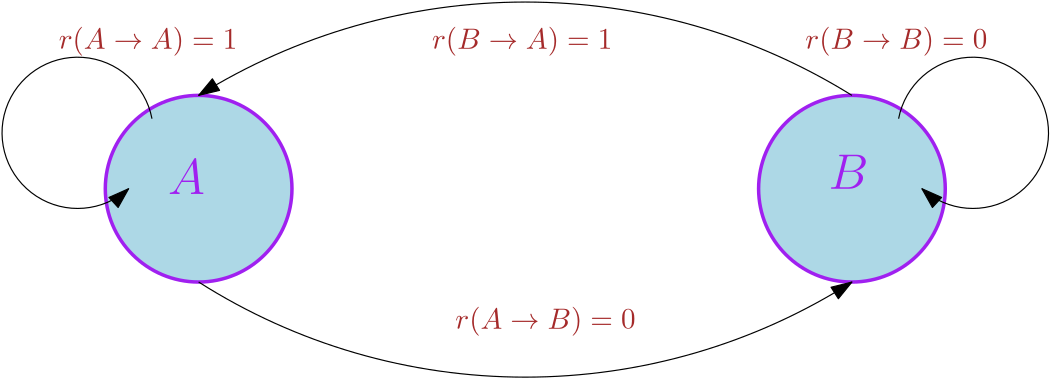
\includegraphics[width=0.6\linewidth]{figs/mdp_2state.png}
  \end{center}
  \vspace{8pt}
In other words, we have $\mathcal{S}=\{A,B\}$, $\mathcal{A}=\{\text{switch}, \text{stay}\}$,
$$
r(A,\text{switch})=0, r(A,\text{stay})=1, r(B,\text{switch})=1, r(B,\text{stay})=0,
$$
$$
P(A|A,\text{switch})=0, P(A|A,\text{stay})=1, P(B|B,\text{switch})=0, P(B|B,\text{stay})=1.
$$
Let $\gamma\in(0,1)$ be the discount factor. Let optimal policy be $\pi_{opt}$ which is the policy that always goes to A (see HW1).
\begin{questions}
    \question[10] Consider the policy class parametrized by two parameters: $\pi(\text{stay} | A) = \theta_1$ and $\pi(\text{switch} | B) = \theta_2$ with $\theta_1, \theta_2\in[0,1]$. Let $\boldsymbol{\theta} = (\theta_2, \theta_2)$. 
    \begin{enumerate}
        \item Compute the value function $V^{\pi(\boldsymbol{\theta})}(A)$ and  $V^{\pi(\boldsymbol{\theta})}(B)$.
        \item  Are $V^{\pi(\boldsymbol{\theta})}(A)$ and $V^{\pi(\boldsymbol{\theta})}(B)$ concave in $\boldsymbol{\theta}$ when $\theta_1, \theta_2\in[0,1]$?
        \item Does the policy gradient with stepsize small enough always converge to $\pi_{opt}$  by maximizing $V^{\pi(\boldsymbol{\theta})}(A)$? Does the policy gradient with stepsize small enough always converge to $\pi_{opt}$  by maximizing $V^{\pi(\boldsymbol{\theta})}(B)$?
        %\item Plot the trajectory of policy gradient with $\gamma =0.9$.
    \end{enumerate}
    \question[10] Consider the policy class parametrized by one parameter: $\pi(\text{stay} | A) = \pi(\text{switch} | B) = \theta$ with $\theta\in[0,1]$.  
    \begin{enumerate}
        \item Compute the value function $V^{\pi(\theta)}(A)$ and  $V^{\pi(\theta)}(B)$.
        \item Are $V^{\pi(\theta)}(A)$ and $V^{\pi(\theta)}(B)$ concave in $\theta$ when $\theta\in[0,1]$? 
        \item Does the policy gradient with stepsize small enough always converge to $\pi_{opt}$ by maximizing $V^{\pi(\theta)}(A)$? Does the policy gradient with stepsize small enough always  converge to $\pi_{opt}$  by maximizing $V^{\pi(\theta)}(B)$?
    \end{enumerate}
    \question[5] Consider the policy class parametrized by one parameter: $\pi(\text{stay} | A) = \pi(\text{switch} | B) = \left(\theta-\frac{1}{4}\right)^2$ with $\theta\in[0,\frac{5}{4}]$. Does the policy gradient with stepsize small enough always converge to $\pi_{opt}$  by maximizing $V^{\pi(\theta)}(B)$?
\end{questions}

\paragraph{Remark.} With different parameterizations, the value function can be concave or nonconcave. Under restricted policy class even if it contains the optimal policy, policy gradient may not always find the optimal policy.\\



Contact: \texttt{junchi.yang@inf.ethz.ch}

\begin{Solution}
    \begin{enumerate} [label=\alph*)]
        \item
        1. Solve the Bellman Consistency Equation for states $A$ and $B$
        $$
        \begin{aligned}
        V^{\pi_\theta}(A) & = \pi_\theta (\text{stay} \mid A) (r(A, \text{stay}) + \gamma V^{\pi_\theta}(A)) + \pi_\theta (\text{switch} \mid A) (r(A, \text{switch}) + \gamma V^{\pi_\theta}(B)) \\
        & = \theta_1 (1 + \gamma V^{\pi_\theta}(A)) + (1 - \theta_1)(0 + \gamma V^{\pi_\theta}(B)) \\
        V^{\pi_\theta}(B) & = \pi_\theta (\text{stay} \mid B) (r(B, \text{stay}) + \gamma V^{\pi_\theta}(B)) + \pi_\theta (\text{switch} \mid B) (r(B, \text{switch}) + \gamma V^{\pi_\theta}(A)) \\
        & = (1 - \theta_2)(0 + \gamma V^{\pi_\theta}(B)) + \theta_2 (1 + \gamma V^{\pi_\theta}(A))
        \end{aligned}
        $$
        Note that $\gamma \in (0,1)$ and $\theta_1, \theta_2 \in [0,1]$, we have
        $$
        V^{\pi_\theta}(A) = \dfrac{(1 - \gamma) \theta_1 + \gamma \theta_2}{(1 - \gamma)(1 - \gamma (\theta_1 - \theta_2))}, \quad 
        V^{\pi_\theta}(B) = \dfrac{\theta_2}{(1 - \gamma)(1 - \gamma (\theta_1 - \theta_2))}
        $$
        \vspace{1em}
        
        2. To determined the concavity of the value functions, we can fix one coordinate while varying the other. In this manner, we observe that both the value functions $V^{\pi_\theta}(A)$ and $V^{\pi_\theta}(B)$ show convexity with respect to $\theta_1$ in particular when $\theta_2$ is close to zero.
        
        For example, let $\gamma = 0.9$ and fix $\theta_2 = 0.1$, we have
        $$
        V^{\pi_\theta}(s) \mid_{\theta_1 = 0.5, \theta_2 = 0.1} \leq \dfrac{1}{2} \automedpar{V^{\pi_\theta}(s) \mid_{\theta_1 = 0, \theta_2 = 0.1} + V^{\pi_\theta}(s) \mid_{\theta_1 = 1, \theta_2 = 0.1}}, \quad \forall s \in \{A, B\}
        $$
        
        Therefore we conclude that $V^{\pi_\theta}(A)$ and $V^{\pi_\theta}(B)$ are not concave.
        
        This conclusion can be also verified by checking the plot of $V^{\pi_\theta}(A)$ and $V^{\pi_\theta}(B)$, which can be easily plotted in 2D case.
        
        \begin{figure}[ht]
        \centering
        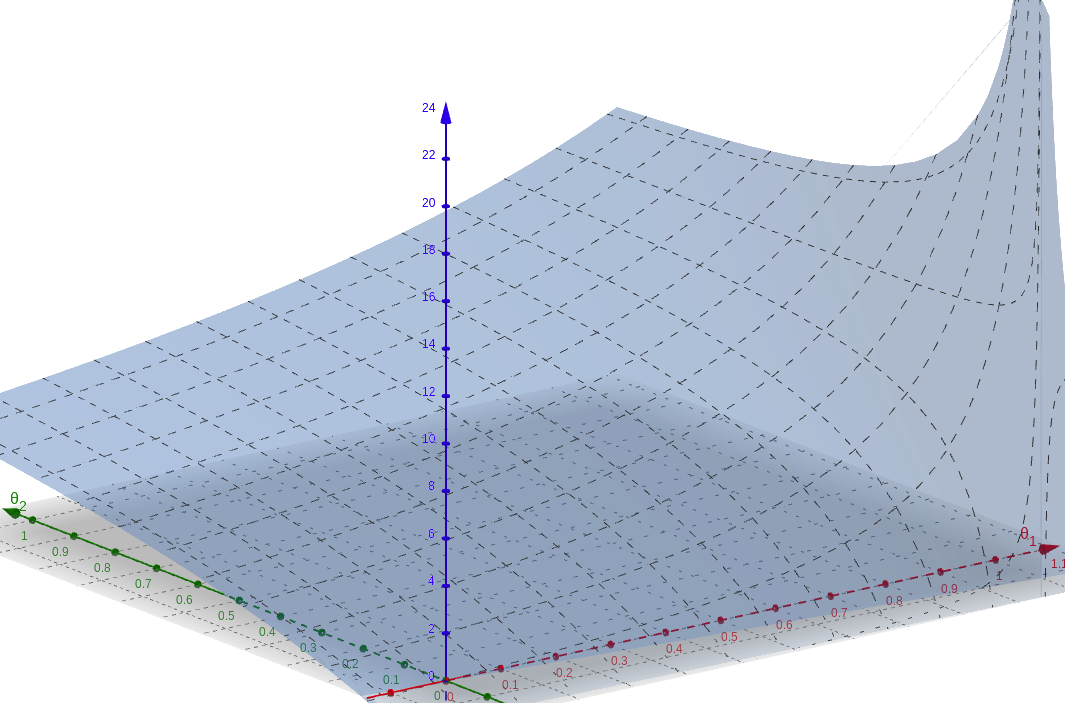
\includegraphics[scale = 0.2]{Assignment 2/figs/a.png} \qquad
        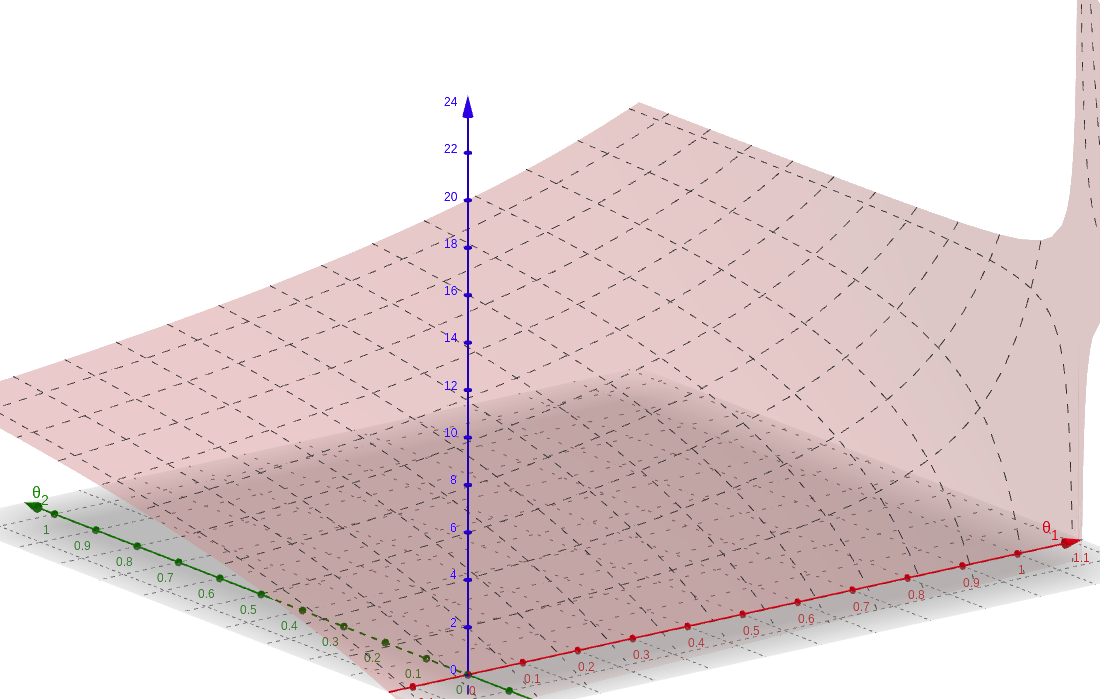
\includegraphics[scale = 0.2]{Assignment 2/figs/b.png}
        \caption{Value functions}
        \label{fig:4_a}
        \end{figure}
        
        In Figure \ref{fig:4_a}, the blue surface corresponds to the value function of $V^{\pi_\theta}(A)$ and the red surface corresponds to the value function of $V^{\pi_\theta}(B)$. And the red and green axis denotes $\theta_1$ and $\theta_2$ respectively. It is obvious that the both surfaces present convexity especially when $\theta_2$ is close to zero. The pictures were captured at the case when $\gamma = 0.9$. However it has been tested that the change of value of $\gamma$ does not affect the concavity of the two value functions.
        \vspace{1em}
        
        3. As $\pi_{opt}(\text{stay} \mid A) = 1$ and $\pi_{opt}(\text{switch} \mid B) = 1$, the optimal value of $\theta_1$ and $\theta_2$ is attained only at the upper bound. Note both $V^{\pi_\theta}(A)$ and $V^{\pi_\theta}(B)$ increase monotonically as $\theta_1$ and $\theta_2$ approach 1. However, observe that $V^{\pi_\theta}(A)$ achieves its maximum at $\theta_1 = 1$ and any $\theta_2 \in [0, 1]$. Therefore the policy gradient with stepsize small enough always converge to $\pi_{opt}$ by maximizing $V^{\pi_\theta}(B)$ but not $V^{\pi_\theta}(A)$.
        
        \item
        1. In this case we can use the conclusion above and set $\theta_1 = \theta_2 = \theta$, we get
        $$
        V^{\pi_\theta}(A) = \dfrac{\theta}{1 - \gamma}, \quad V^{\pi_\theta}(B) = \dfrac{\theta}{1 - \gamma}
        $$
        \vspace{1em}
        
        2. Obviously both $V^{\pi_\theta}(A)$ and $V^{\pi_\theta}(B)$ are linear with respect to $\theta$. Therefore both $V^{\pi_\theta}(A)$ and $V^{\pi_\theta}(B)$ are concave by definition in this case.
        \vspace{1em}
        
        3. Following the previous analysis we know the policy gradient works for both $V^{\pi_\theta}(A)$ and $V^{\pi_\theta}(B)$. Because both value functions are monotonically increasing with respect to $\theta$, we can perform gradient ascent until we hit the upper bound. And therefore the policy gradient with stepsize small enough always converges to $\pi_{opt}$ by maximizing either $V^{\pi_\theta}(A)$ or $V^{\pi_\theta}(B)$.
        
        \item
        From the previous analysis we know that the value function evaluated at $B$ is
        $$
        V^{\pi_\theta}(B) = \dfrac{1}{1 - \gamma}\left (\theta - \dfrac{1}{4} \right )^2
        $$
        which is a convex function with respect to $\theta$. As the optimal value is attained at the boundary, initialization matters in performing gradient ascent. For example, an initialization of $\theta \in [0, \frac{1}{4})$ will eventually lead the algorithm converge to a suboptimal point where $\theta = 0$, whereas the optimal value is attained at $\theta = \frac{5}{4}$. Therefore the policy gradient with stepsize small enough does not necessarily converge to $\pi_{opt}$ by maximizing $V^{\pi_\theta}(B)$.
    \end{enumerate}
\end{Solution}


\clearpage
% %==========================================================================================================

\section{Reading: Q-Learning with Exploration (20 points)}
In the reading exercise, you are expected to read some material and write a paragraph for each question.
The questions may not be well-posed, and are intended to encourage reading and thinking;
the grading here will be more lenient than in the previous problems.
\\

\textbf{Reminder:} As mentioned in \textbf{Instructions}, you should not dig around for homework solutions; if you do rely upon external resources, cite them, and write solutions in your own words. We ask you to follow the ETH Disciplinary Code.
\\

In~\cite{jin2018q} (\href{https://papers.nips.cc/paper/2018/file/d3b1fb02964aa64e257f9f26a31f72cf-Paper.pdf}{NeurIPS 2018 link}), the authors studied the sample complexities of Q-learning algorithms with exploration in tabular episodic MDPs\footnote{As a reminder, because of the finite horizon, different from what we learned in class, here Q-table has a subscript $h$, i.e., each step $h$ has a separate Q-value function.}. Read the paper \cite{jin2018q} and think about the following questions. 

\begin{questions}
\question[2]
The authors mentioned that: ``In episodic MDP, Q-learning with the commonly used $\epsilon$-greedy exploration strategy is can be very inefficient: it can take exponentially many episodes to learn". Similar to Algorithm 1 in \cite{jin2018q}, write out the Q-learning with the $\epsilon$-greedy exploration algorithm in the algorithm environment we provide in the solution part of the {\LaTeX} template.

\question[8]
As shown in Figure \ref{fig:eps-greedy-exp}, there are only two states $ \mathcal{S}=\autobigpar{s_0, s_1} $, the action set $ \mathcal{A} $ may consist of many actions. When staying at $ s_0 $, only $ a^*\in\mathcal{A} $ can keep the state still in $ s_0 $ and the other actions (denoted as $ \mathcal{A}/a^* $ in the figure) will transit to $ s_1 $; when staying at $ s_1 $, any action (denoted as $ \mathcal{A} $ in the figure) keep the state still in $ s_1 $. While the reward function is set as that $ r_H(s_0, a^*)=1 $ and all the others are $ 0 $ (the red arrow in the figure).
    
Show that Q-learning with the $\epsilon$-greedy strategy will be inefficient in this example, i.e., in the worst case, it will take exponentially many episodes to find the optimal policy.
\begin{figure}[htbp]
	\centering
	% include first image
	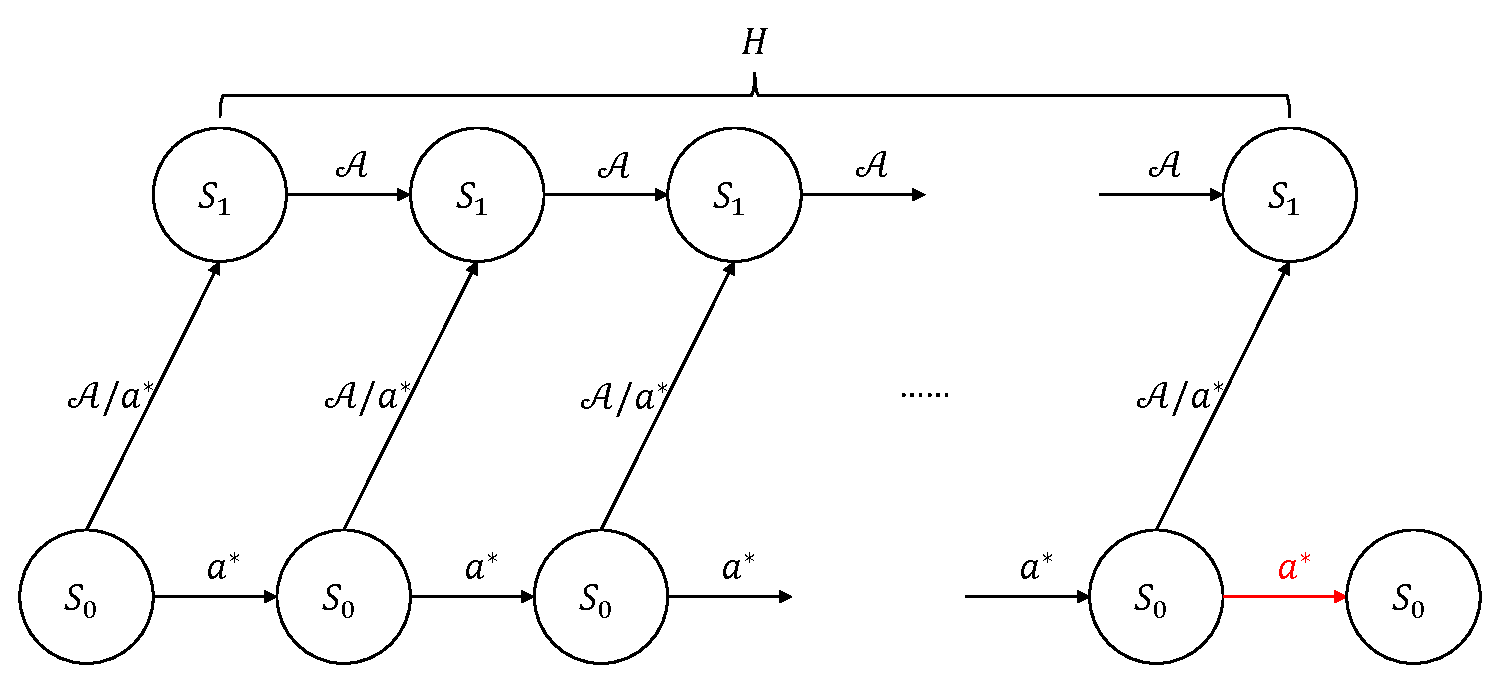
\includegraphics[width=0.7\textwidth]{figs/e-greedy-exp.pdf} 
	\caption{MDP Example}
	\label{fig:eps-greedy-exp}
\end{figure}

\question[10] 
Q-learning is an important algorithm in model-free RL algorithms. With this paper:
\begin{itemize}
    \item[1.] What is your take-away from this paper? (3 points)
    \item[2.] Do you think the result in the paper is important? Why? (3 points)
    \item[3.] What is the main limitation of the paper? (4 points)
\end{itemize}

\end{questions}

Contact: \texttt{siqi.zhang@inf.ethz.ch}


\begin{Solution}
    \begin{enumerate} [label=\alph*)]
        \item
        The Q-learning with the $\epsilon$-greedy exploration algorithm follows
        \begin{algorithm}[H]
    	\caption{Q-learning with $\epsilon$-greedy exploration}
    	\color{blue}
    	\begin{algorithmic}[1]
    		\REQUIRE Initialize $Q_h(s,a)$ for all $(x,a,h)\in\mathcal{S}\times\mathcal{A}\times[H]$
            \FORALL{episodes $k = 1,2,...,K$}
                \STATE Initialize $s \in \mathcal{S}$
                \FORALL{step $h = 1,2,...,H$}
                    \STATE $a \leftarrow
                    \begin{cases} \argmax_{a \in \mathcal{A}} Q_h(s,a) & \text { with probability } 1-\epsilon \\
                    \text{Uniform}(\mathcal{A}) & \text { with probability } \epsilon
                    \end{cases}
                    $
                    \STATE Take action $a$, observe reward $r$ and next state $s'$
                    \STATE
                    $
                    Q_h(s,a) \leftarrow Q_h(s,a) + \alpha \automedpar{r + \gamma \max_{a' \in \mathcal{A}} Q_h(s', a') - Q_h(s,a)}
                    $
                    \STATE $ s \leftarrow s' $
                \ENDFOR
                \ENDFOR
    	    \end{algorithmic}
        \end{algorithm}
        
        \item
        In this setting the agent only gets reward $ r_H(s_0, a^*)=1 $ at the end of the episode. This means the optimal policy is to always act $a^*$ so as to keep the state at $s_0$ to the end. There are in total $|\mathcal{A}|^H$ many episodes (as each action sequence uniquely determines an episode) but only the one with $a_h = a^*$ for all $h \in H$ generates a non-zero return.
        
        In this case, the policy stays completely random before the Q-learning with the $\epsilon$-greedy exploration algorithm samples the only rewarding episode, as all $Q_h(s,a)$ stays at zero for all $s \in \mathcal{S}$, $a \in \mathcal{A}$ and $h \in [H]$. The only hope to arrive the only rewarding episode is by uniformly random sampling with probability $\dfrac{1}{|\mathcal{A}|^H}$.
        
        The computational time to collect $r_H(s_0, a^*)$ is  $\mathcal{O}(|\mathcal{A}|^H)$. However, even after the algorithm has finally achieved this immediate reward at the end, only $Q_H(s_0, a^*)$ turns non-zero. In like manner, it will take $\mathcal{O}(|\mathcal{A}|^{H-1})$ time to reach this value function. Therefore, it will take $\mathcal{O}(\sum_{h=1}^H |\mathcal{A}|^h)$ time for the algorithm to populate this reward at the end of the episode all the way to the beginning. This is greatly inefficient and therefore in the worst case the algorithm will take exponentially many episodes to find the optimal policy.
        
        \item
        1.
        Standard Q-learning heuristic of incorporating $\epsilon$-greedy exploration can take exponentially many episodes to learn the optimal policy, which is extremely inefficient in some cases. However, when equipped with a upper confidence bounds (UCB) exploration policy that incorporates estimates of the confidence of Q values and assign exploration bonuses, Q-learning can achieve total regret $\~{\mathcal{O}}(H^3 SAT)$. This is a great improvement on the sample efficiency of model-free algorithms which are empirically considered to be sample inefficient compared with model-based methods. Thus, the proposed Q-learning method enjoys both advantages over model-free algorithms in terms of simplicity and flexibility and model-based algorithms in terms of time and space complexities.
        
        As mentioned by the authors, the proposed learning rate of $\alpha_t = \mathcal{O}(H/t)$ when a state-action pair is being updated for the $t$-th time plays a crucial role in obtaining regret that is not exponential in $H$. The specific choice of learning rate assigns more weight to updates that are more recent, as opposed to assigning uniform weights to all previous updates as used in common cases.
        \vspace{1em}
        
        2.
        I think the result presented in the paper is very important and meaningful. As discussed in the previous part, the great improvement of sample efficiency of Q-learning as a model-free algorithm using the proposed UCB exploration method incorporating Q value confidence and exploration bonuses gives an answer to the fundamental question in terms of the intrinsic inefficiency problems of model-free algorithms in reinforcement learning. This could significantly change the pattern of application of model-free and model-based methods today. As the proposed Q-learning method enjoys both advantages over model-free algorithms in terms of simplicity, flexibility and online computation and also model-based algorithms in terms of time and space complexities, it promotes the idea that model-free methods are comparable to model-based methods in terms of sample efficiency, which was thought to be limiting its applications.
        \vspace{1em}
        
        3.
        This paper limits its focus on tabular episodic Markov decision process settings where the numbers of states and actions are finite. Therefore, it has not been proved that the result could be adapted to the continuous state and action space.
        
        As reported in the paper, the Q-learning with both Hoeffding-style bonus and Bernstein-style bonus has an asymptotic regret dependency on episode steps $H$. This result in lower efficiencies than the regret achieved by model-based algorithms in the case where the episode length is rather large.
    \end{enumerate}



\end{Solution}

\clearpage

%\input{solutions}

\bibliographystyle{plain}
\bibliography{references}

\end{document}
